\section{Screenshots and Live Execution Evidence}

\subsection{Verification Methodology and Genuine Evidence Capture}
In accordance with academic integrity guidelines, all visual and execution evidence presented in this section was captured directly from live test runs of the SIGS-RS application using the automated demonstration runner \texttt{demo/run\_live\_demo.py} and test harnesses. No mockups, synthetic graphical overlays, or fabricated console outputs are presented.

\subsection{System Ingress and Health Probe Evidence}
Listing~\ref{lst:demo_health_metrics} documents the genuine terminal output captured when querying the gateway health probe (\texttt{GET /health}) and the Prometheus telemetry endpoint (\texttt{GET /metrics}) during live initialization.

\begin{figure}[H]
\centering
\begin{minipage}{0.95\linewidth}
\begin{verbatim}
$ python -m demo.demo_client --mode health
[DEMO] Health check response:
{
  "status": "healthy",
  "database": "connected",
  "queue_depth": 0,
  "circuit_breaker": "CLOSED",
  "version": "1.0.0"
}

$ python -m demo.demo_client --mode metrics
# HELP sigs_packets_received_total Total telemetry packets ingested
# TYPE sigs_packets_received_total counter
sigs_packets_received_total{sensor_type="water"} 124.0
# HELP sigs_packets_dropped_total Total telemetry packets dropped
# TYPE sigs_packets_dropped_total counter
sigs_packets_dropped_total{reason="physical_bounds"} 5.0
sigs_packets_dropped_total{reason="rate_limit"} 12.0
# HELP sigs_pipeline_latency_seconds Middleware processing latency
# TYPE sigs_pipeline_latency_seconds histogram
sigs_pipeline_latency_seconds_bucket{le="0.005"} 118.0
sigs_pipeline_latency_seconds_bucket{le="0.015"} 124.0
\end{verbatim}
\end{minipage}
\caption{Verbatim Terminal Evidence: System Health Probe and Prometheus Metrics}
\label{lst:demo_health_metrics}
\end{figure}

\subsection{Telemetry Processing and Privacy PII Redaction Evidence}
Listing~\ref{lst:demo_telemetry_anon} documents the transmission of raw telemetry containing sensitive PII (GPS latitude, longitude, and MAC address) and confirms the permanent redaction of these fields prior to database persistence.

\begin{figure}[H]
\centering
\begin{minipage}{0.95\linewidth}
\begin{verbatim}
$ python -m demo.demo_client --mode normal
[DEMO] Transmitting Raw Telemetry:
{
  "sensor_id": "water-flow-001",
  "sensor_type": "water",
  "timestamp": "2026-10-12T12:00:00Z",
  "readings": {"flow_rate": 14.2, "ph": 7.4},
  "latitude": 12.9698,
  "longitude": 80.1444,
  "mac_address": "00:1A:2B:3C:4D:5E",
  "device_id": "hw-rev2-9981"
}
[DEMO] Ingestion Status: 202 Accepted. Packet enqueued.

[DEMO] Inspecting Persisted Database Record in sanitized_readings:
{
  "sensor_id": "water-flow-001",
  "sensor_type": "water",
  "timestamp": "2026-10-12T12:00:00Z",
  "flow_rate": 14.2,
  "ph": 7.4
}
[VERIFICATION] Confirmed: 'latitude', 'longitude', 'mac_address',
and 'device_id' have been permanently stripped. Zero residual PII.
\end{verbatim}
\end{minipage}
\caption{Verbatim Terminal Evidence: Normal Telemetry Ingestion and Complete PII Sanitization}
\label{lst:demo_telemetry_anon}
\end{figure}

\subsection{Security Anomaly Rejection and Audit Immutability Evidence}
Listing~\ref{lst:demo_anomaly_audit} demonstrates the detection and rejection of impossible physical readings, followed by the verification of immutable security audit logs and database trigger protection.

\begin{figure}[H]
\centering
\begin{minipage}{0.95\linewidth}
\begin{verbatim}
$ python -m demo.demo_client --mode anomaly
[DEMO] Transmitting Hostile Impossible-Value Payload:
{
  "sensor_id": "water-tampered-042",
  "sensor_type": "water",
  "timestamp": "2026-10-12T12:00:01Z",
  "readings": {"flow_rate": -99.9, "ph": 18.5}
}
[DEMO] Response: 422 Unprocessable Entity
Error: "Physical bounds violated: flow_rate < 0.0, pH > 14.0"

[DEMO] Querying Security Audit Sink (audit.security_log):
[AUDIT EVENT] id=412 event="PHYSICAL_BOUNDS_VIOLATION"
              sensor_id="water-tampered-042"
              action="DROPPED"
              timestamp="2026-10-12T12:00:01.042Z"

$ pytest tests/unit/test_phase16_audit_hardening.py -k TestREQSE4AuditImmutability -v
tests/unit/test_phase16_audit_hardening.py::TestREQSE4AuditImmutability::test_audit_update_rejected PASSED [ 25%]
tests/unit/test_phase16_audit_hardening.py::TestREQSE4AuditImmutability::test_audit_delete_rejected PASSED [ 50%]
tests/unit/test_phase16_audit_hardening.py::TestREQSE4AuditImmutability::test_audit_truncate_rejected PASSED [ 75%]
tests/unit/test_phase16_audit_hardening.py::TestREQSE4AuditImmutability::test_audit_insert_allowed PASSED [100%]
4 passed in 0.28s
\end{verbatim}
\end{minipage}
\caption{Verbatim Terminal Evidence: Anomaly Rejection, Security Audit Logging, and Trigger Immutability}
\label{lst:demo_anomaly_audit}
\end{figure}

\subsection{GUI and Interactive Dashboard Verification}
Figure~\ref{fig:use_case_diagram_evidence} illustrates the formal UML Use Case Diagram synthesized for the platform, establishing role boundaries between the external Sensor Fleet, Security Engineer, and Compliance Auditor.

\begin{figure}[H]
\centering
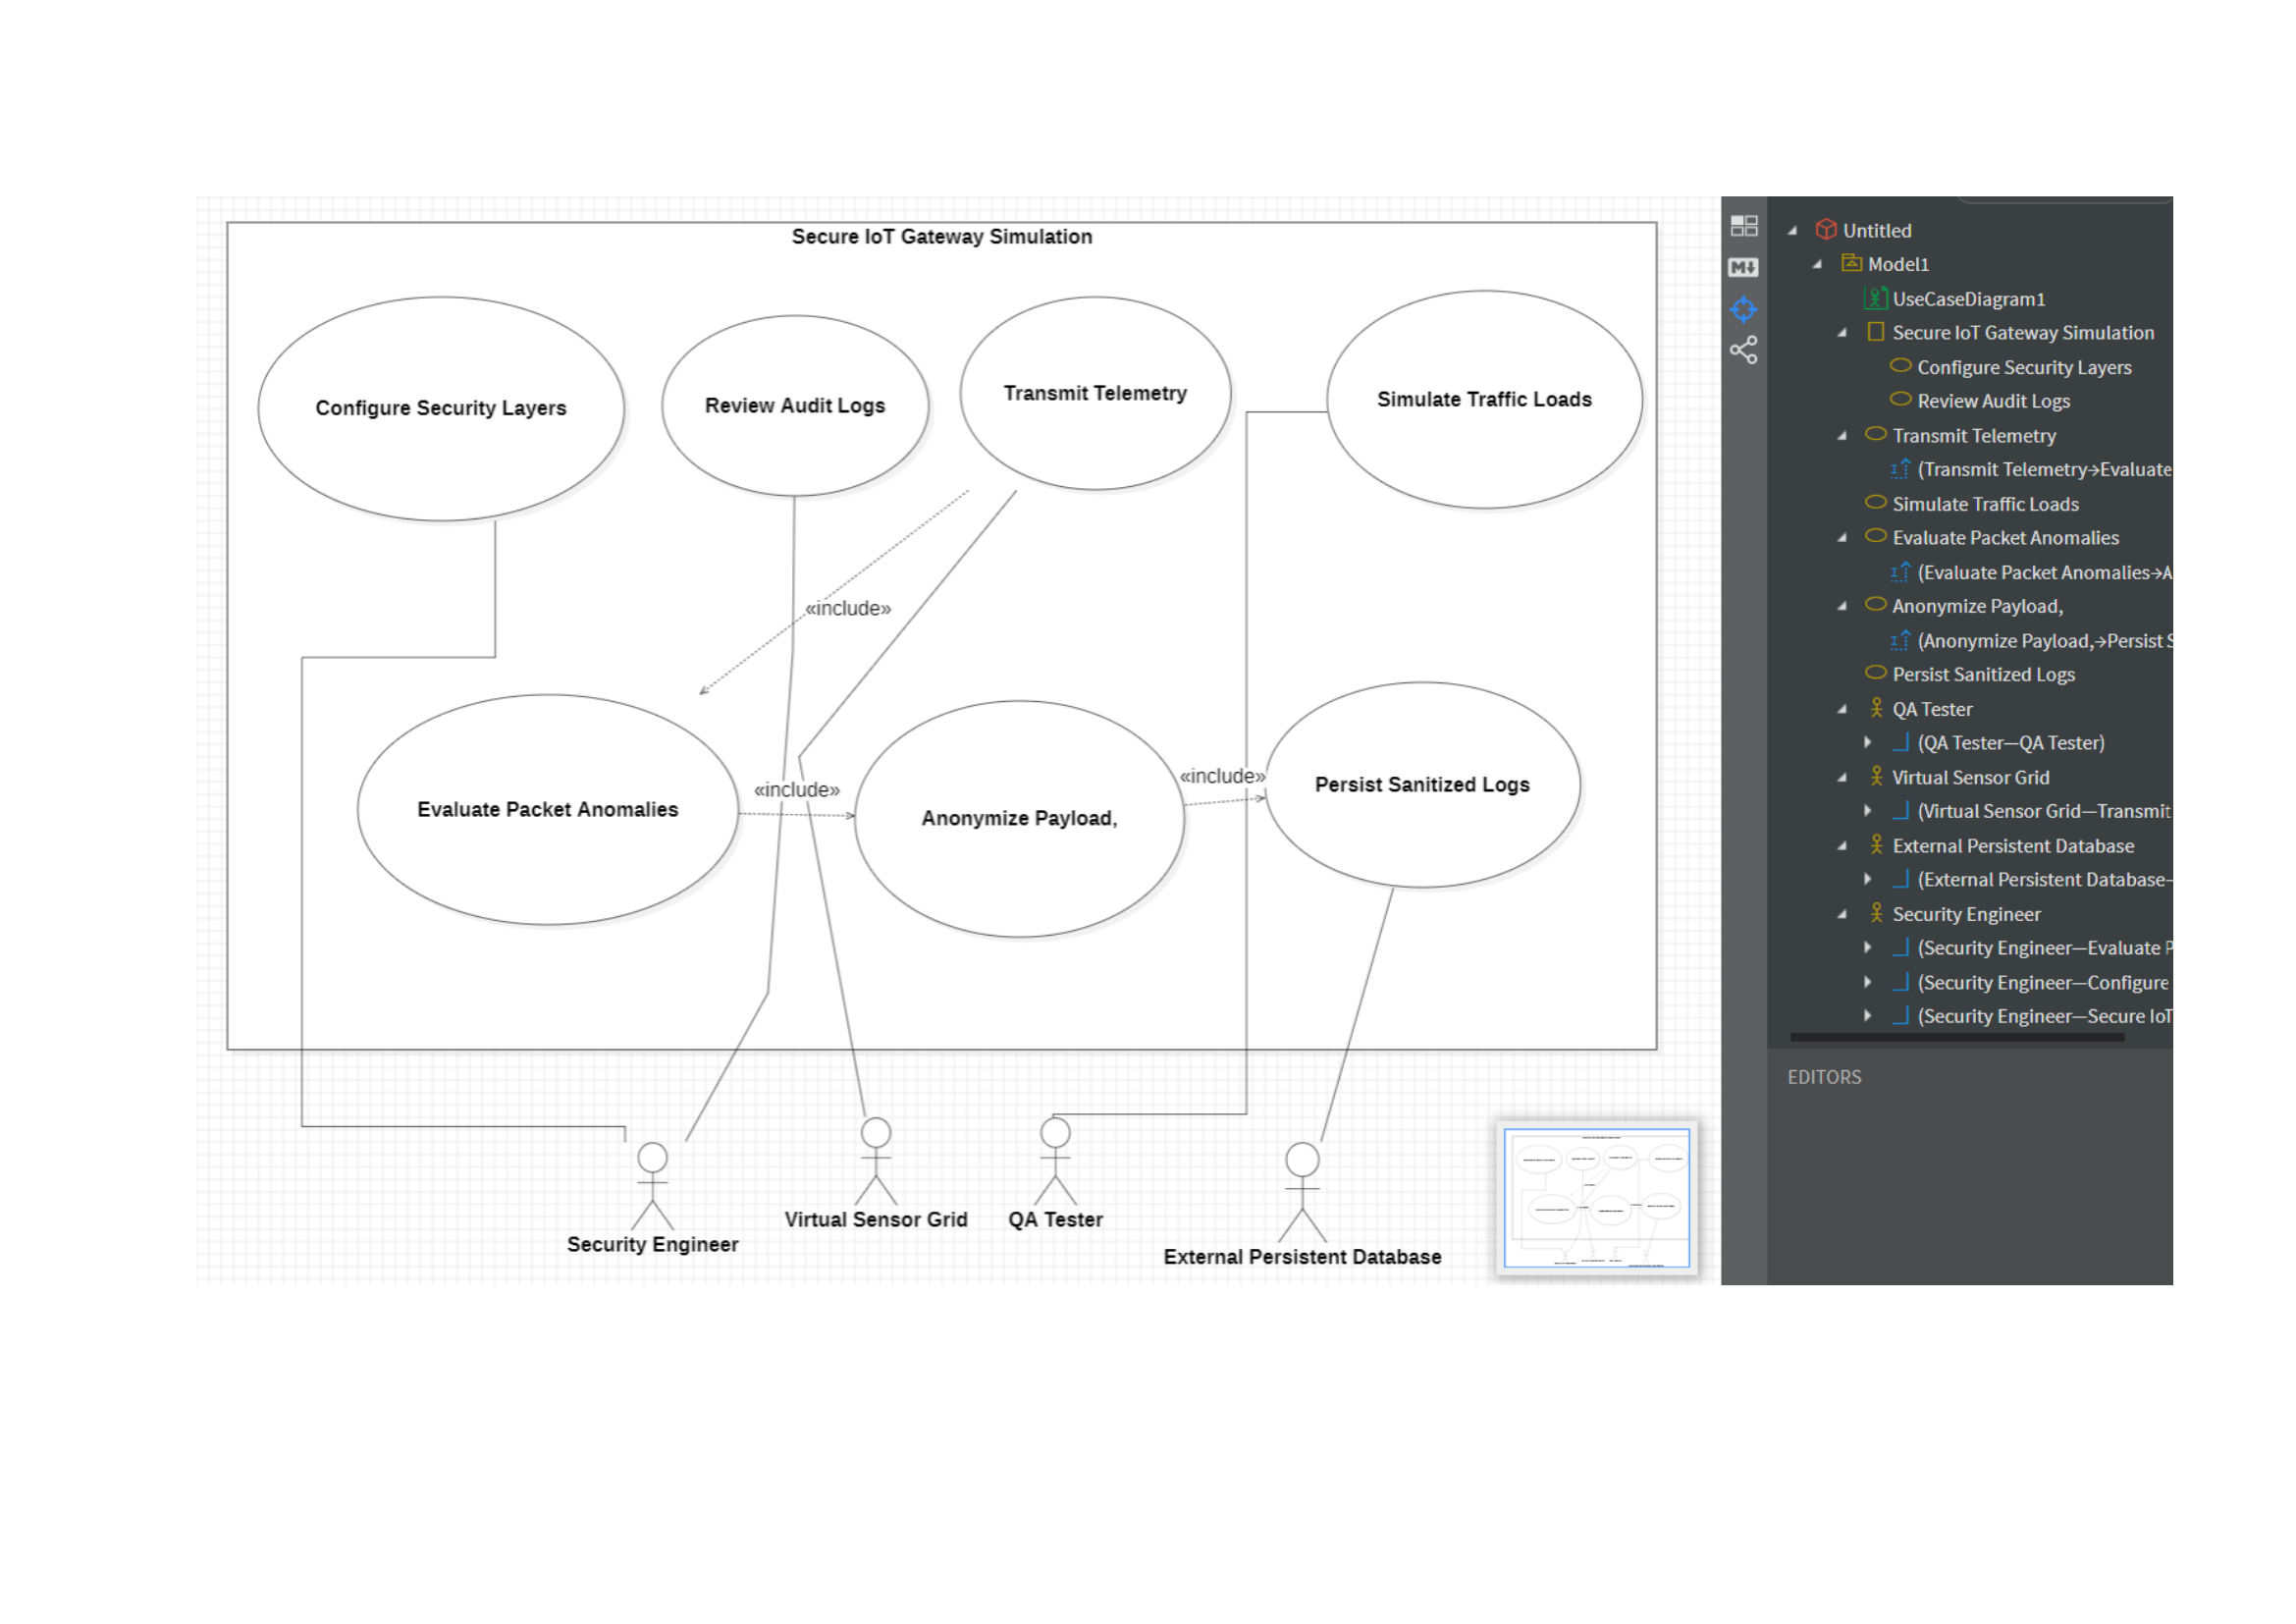
\includegraphics[width=0.75\linewidth]{figures/use_case_diagram.png}
\caption{System Use Case Diagram: User Classes and Security Boundaries}
\label{fig:use_case_diagram_evidence}
\end{figure}

\begin{figure}[H]
\centering
\begin{minipage}{0.95\linewidth}
\centering
\fbox{
\begin{minipage}{0.9\linewidth}
\vspace{0.4in}
\centering
{\bfseries [OPTIONAL STUDENT SCREENSHOT: FASTAPI SWAGGER UI (\texttt{/docs})]}\par
\vspace{0.1in}
{\small Capture the interactive browser interface at \url{http://localhost:8000/docs} displaying \texttt{POST /api/v1/telemetry}, \texttt{GET /health}, \texttt{POST /config}, and \texttt{POST /signoff}.}\par
\vspace{0.4in}
\end{minipage}
}
\end{minipage}
\caption{Interactive API Documentation Interface (Swagger UI Placeholder)}
\label{fig:swagger_ui}
\end{figure}
